\documentclass[tikz,border=4pt,11pt]{standalone}
\usepackage{amsmath}
\definecolor{ink}{RGB}{42,52,64}
\definecolor{first}{RGB}{146,79,26}
\definecolor{second}{RGB}{26,99,111}

% The Pieri rules for lambda = (2,1), English notation.  Top row: the four
% horizontal strips of size two added to (2,1), giving
% h_2 s_21 = s_41 + s_32 + s_311 + s_221.  Bottom row: the four vertical
% strips, giving e_2 s_21 = s_32 + s_311 + s_221 + s_2111.
% The cells of (2,1) are white, the added cells are shaded.

\begin{document}
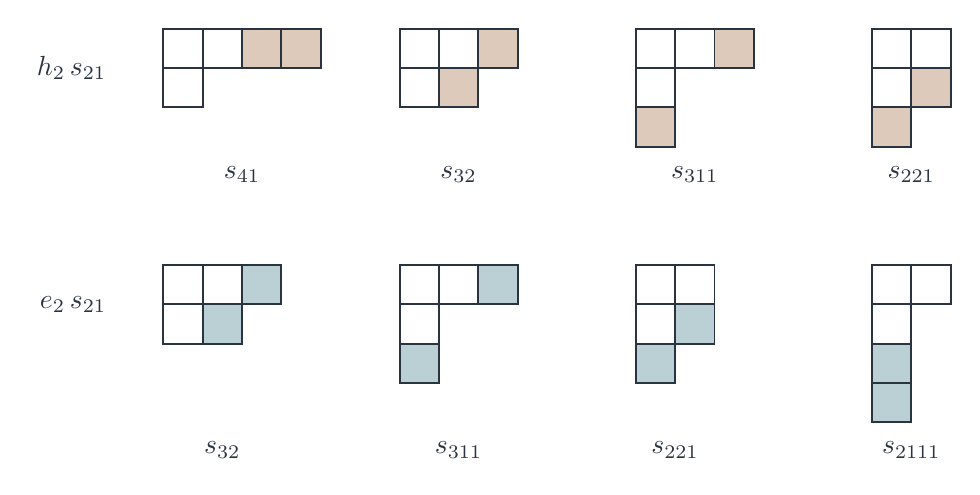
\begin{tikzpicture}[text=ink,x=.5cm,y=.5cm]
% \young{row lengths of mu}{added cells (col/row), 1-indexed}{colour}{label}{x of label}
% The label is placed below the row of diagrams, at height \laby.
\newcommand{\young}[5]{%
  \foreach \c/\r in {#2} \fill[#3!30] (\c-1,-\r) rectangle (\c,-\r+1);
  \foreach \r/\len in {#1}
    \foreach \c in {1,...,\len}
      \draw[ink,line width=.7pt] (\c-1,-\r) rectangle (\c,-\r+1);
  \node[anchor=north] at (#5,\laby) {$#4$};
}

\def\laby{-3.25}
\node[anchor=east] at (-1.2,-1) {$h_2\,s_{21}$};
\begin{scope}[shift={(0,0)}]\young{1/4,2/1}{3/1,4/1}{first}{s_{41}}{2.0}\end{scope}
\begin{scope}[shift={(6,0)}]\young{1/3,2/2}{3/1,2/2}{first}{s_{32}}{1.5}\end{scope}
\begin{scope}[shift={(12,0)}]\young{1/3,2/1,3/1}{3/1,1/3}{first}{s_{311}}{1.5}\end{scope}
\begin{scope}[shift={(18,0)}]\young{1/2,2/2,3/1}{2/2,1/3}{first}{s_{221}}{1.0}\end{scope}

\def\laby{-4.25}
\node[anchor=east] at (-1.2,-7) {$e_2\,s_{21}$};
\begin{scope}[shift={(0,-6)}]\young{1/3,2/2}{3/1,2/2}{second}{s_{32}}{1.5}\end{scope}
\begin{scope}[shift={(6,-6)}]\young{1/3,2/1,3/1}{3/1,1/3}{second}{s_{311}}{1.5}\end{scope}
\begin{scope}[shift={(12,-6)}]\young{1/2,2/2,3/1}{2/2,1/3}{second}{s_{221}}{1.0}\end{scope}
\begin{scope}[shift={(18,-6)}]\young{1/2,2/1,3/1,4/1}{1/3,1/4}{second}{s_{2111}}{1.0}\end{scope}
\end{tikzpicture}
\end{document}
